\section{Redes fractales}

Los fractales en naturaleza son estructuras que mantienen su forma a diferentes escalas. En el caso de las redes, existe una familia conocida como $(x,y)-$flowers\cite{Rozenfeld2007}, la cuales son conocidas como redes libres de escala jerárquicas. Rozenfeld y otros\cite{Rozenfeld2007B} han demostrado analíticamente que estas redes conservan sus propiedades analizando el escalado de los hubs y los nodos.

Un método de construcción iterativo de estas redes es propuesto por Lin y otros\cite{Lin2011} en un estudio de árboles de cobertura mínima en redes complejas autosimilares.

Este método, consiste en generar una función $F(x,y)$ donde $x>0$ y $y>0$ que permite construir la flor dadas $n$ generaciones. Para $n=0$ la red que genera $F_0(x,y)$ siempre tiene dos vértices unidos por una arista.  A medida que se itera $F_n(x,y)$ se deriva al reemplazar cada arista existente en $F_{n-1}$ por caminos de largo $x$ e $y$. El número de aristas del algoritmo generador siempre es $|E| = (x+y)^n$. 

\begin{figure}[H]
    \centering
    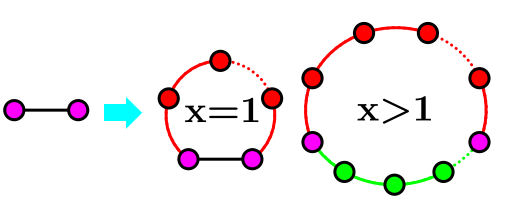
\includegraphics[scale=0.5]{Capitulo3GeneracionRedesFractales/imagenes/florA.png}
    \caption{Proceso iterativo de construcción de las $(x-y)$-flowers. Tomado de \cite{Lin2011}}
    \label{fig:floarA}
\end{figure}

En la figura \ref{fig:floarA} el proceso iterativo consiste en reemplazar cada arista con un camino de tamaño $x, x\leq 1$ y $y, y\leq x \wedge y > 1$. Para $x=1$ un par de nodos de la iteración anterior es directamente conectado con $y-1$ nuevos nodos. Todos estos nuevos nodos y dos de los nodos de la iteración anterior forma un camino rojo de tamaño $y$. Para $x>1$ cada arista antigua es reemplazada por dos caminos que consisten en $y-1$ nodos.

Otra forma de construir las redes es ir formando la red con copias de ella misma. En la figura \ref{fig:florGeneradas} se observa este proceso.

\begin{figure}[H]
    \centering
    \begin{subfigure}[b]{0.5\textwidth}
        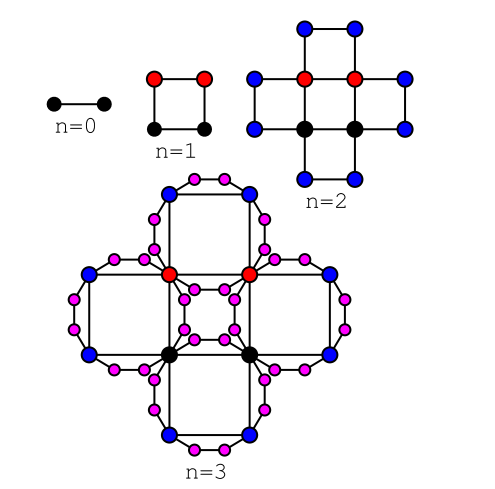
\includegraphics[width=\textwidth]{Capitulo3GeneracionRedesFractales/imagenes/florB.png}
        \caption{Generación de $(1,3)-$flower}
    \end{subfigure}~
    \begin{subfigure}[b]{0.5\textwidth}
        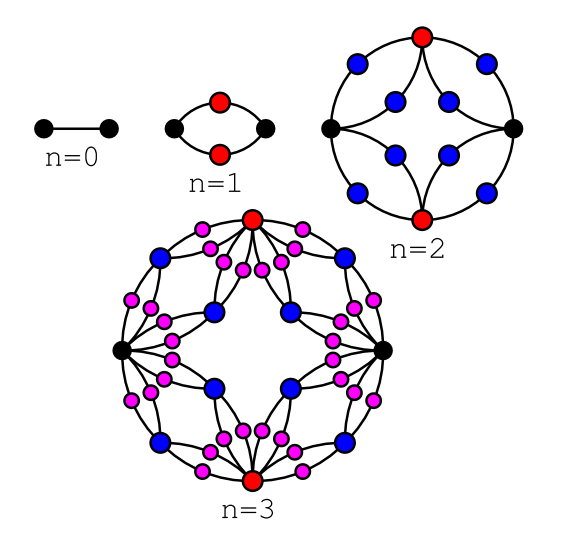
\includegraphics[width=\textwidth]{Capitulo3GeneracionRedesFractales/imagenes/florC.png}
        \caption{Generación de $(2,2)-$flower} 
    \end{subfigure}
    \caption{Proceso iterativo de generación de redes $(x,y)$-flowers. Tomado de \cite{Lin2011}}
    \label{fig:florGeneradas}
\end{figure}